\subsection{Relaciones Dinámicas}

Las relaciones dinámicas describen las dependencias temporales entre los elementos de la arquitectura. Se distinguen dos tipos de relaciones dinámicas: de activación y de flujo.

\begin{table}[h]
	\subsubsection{Elementos}
	\begin{center}
		\begin{tabular}{| l | l | r |}
			\hline
			Concepto & Descripción & Representación \\ \hline
			
			Flujo 
			&
			\begin{tabular}[l]{@{}l@{}}
				Transferencia de un elemento a otro.
			\end{tabular}
			& 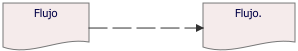
\includegraphics[width=0.4\linewidth]{imgs/relaciones/flujo}
			\\\hline
			
			Disparo
			& 
			\begin{tabular}[l]{@{}l@{}}
				Describe una relación temporal o \\
				causal entre los elementos.
			\end{tabular}
			& \includegraphics[width=0.4\linewidth]{imgs/relaciones/disparo}
			\\\hline
			
		\end{tabular}
		\caption{Relaciones dinámicas}
		\label{tab:dinamicas}
	\end{center}
\end{table}
